\chapter{Transversality and Intersection}

\section{Manifolds with Boundary}

Our previous study does not account for all geometric objects, mainly those that possess \textit{boundaries}, like the closed unit ball or the cylinder $S^1 \times [0,1]$. Neighbourhoods of points on the boundary are not diffeomorphic to any open set in $\R^n$, so we need to account for this. 

\subsection{Definition}

The simplest example of a manifold with boundary is the upper half-space $H^k$ in $\R^k$, the set of points in $\R^k$ with nonnegative final coordinate, with boundary $\R^{k-1}$ with the usual embedding into $\R^k$. This will be the model that we use to define a general manifold with boundary. 

\begin{definition}
    $X \subseteq \R^N$ is a $k$-dimensional \textbf{manifold with boundary} if every point of $X$ posesses a neighbourhood diffeomorphic to an open set in $H^k$. We call this diffeomorphism a \textbf{local parameterization} of $X$. 

    The \textbf{boundary} of $X$, denoted $\partial X$, is the set of points belonging to the image of the boundary of $H^k$ under a local parameterization. The complement of the boundary is called the \textbf{interior}, denoted $Int(X)$.
\end{definition}

\begin{center}
    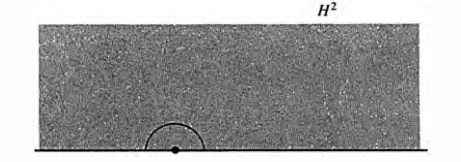
\includegraphics[width=0.6\textwidth]{Chapters/upper half plane.png}
\end{center}

\begin{remark}
    Do not confuse these definitions with the topological boundary or interior of $X$. While these do agree if $\dim X = N$, they definitely don't if $\dim X < N$. 

    All manifolds defined earlier are manifolds with boundary, and have empty boundaries. We will still call them just ``manifolds.''
\end{remark}

Note that certain properties established in Chapter 1 do not apply to manifolds with boundary. For example, the product of two manifolds with boundary is not always a manifold with boundary. To see this, consider $[0,1]$. Then the square $[0,1] \times [0,1]$ is not a manifold with boundary because the corners of the square are sharp, and hence we cannot attain a local parameterization at the corners. Despite this, we still get some interesting results in this area:

\begin{prop}
    The product of a manifold without boundary $X$ and a manifold with boundary $Y$ is a manifold with boundary. Moreover, we have 
    \[\partial (X \times Y) = X \times \partial Y, \quad \text{ and } \quad \dim (X \times Y) = \dim X + \dim Y\]
\end{prop}

\begin{proof}
    Let $U \subset \R^k, V \subset H^l$ be open. Then 
    \[U \times V \subset \R^k \times H^l = H^{k+l}\]
    is open. Moreover, if $\phi: U \to X$ and $\psi: V \to Y$ are local parameterizations, so is $\phi \times \psi: U \times V \to X \times Y$. 
\end{proof}

This result will come in handy later when considering the homotopy mapping space $X \times I$ of some manifold $X$. 

$Int(X)$ is a boundaryless manifold of the same dimension as $X$, since all interior points in the range of a local parameterization with domain an open set of $H^k$ contained entirely in the interior is an open set of $\R^k$. More interestingly,

\begin{prop}
    If $X$ is a $k$-dimensional manifold with boundary, then $\partial X$ is a $(k-1)$-dimensional manifold without boundary. 
\end{prop}

\begin{proof}
    Let $x \in \partial X$. Then there is a local parameterization $\phi: U \to V$, where $U$ is open in $H^k$ and $V$ open in $X$. It suffices to show that $\phi(\partial U) = \partial V$, as if so, we may restrict $\phi$ to a diffeomorphism of $\partial U = U \cap \partial H^k$, an open subset of $\R^{k-1}$, with $\partial V = \partial X \cap V$, a neighbourhood of $x \in \partial X$. 

    By definition, we know that $\phi(\partial U) \subset \partial V$, so we only need to prove the reverse. Let $\psi$ be a local parameterization of an open set $W \subset H^k$ into $V$. We claim that $\phi(\partial U) \supset \psi(\partial W)$; equivalently, we show that $\partial U \supset \phi^{-1} \circ \psi(\partial W)$. Let $g = \phi^{-1} \circ \psi: W \to U$, and suppose that $w \in \partial W$ maps to $u \in Int(U)$. $g$ must be a diffeomorphism of $W$ onto some open set $g(W)$ of $U$. Moreover, by the chain rule, we know that $d(g^{-1})_u$ is bijective. But, as $g(w)$ is an interior point, $g(W)$ contains a neighbourhood of $u$ that is open in $\R^k$. By the Inverse Function Theorem applied to $g^{-1}$ on this open set, the image of the inverse contains a neighbourhood of $w$ that is open in $\R^k$. But this would imply that $w$ is an interior point, a contradiction. 
\end{proof}

\subsection{Tangent Spaces and Derivatives}

Tangent spaces and derivatives are still defined on manifolds with boundary. Let $g$ be smooth map from an open set $U \subset H^k$ into $\R^l$. Suppose $u \in U$ is an interior point. Then $dg_u$ is already defined, so we're good on that. If $u \in \partial U$, then as $g$ is smooth, we can extend it to a smooth map $\tilde{g}$ in an open neighbourhood of $u \in \R^k$. From here, define $dg_u$ to be $d\tilde{g}_u: \R^k \to \R^l$. 

We still need to show uniqueness of this derivative. Let $\hat{g}$ be another local extension of $g$. Let $u_i$ be a sequence of points in $Int(U)$ that converge to $u$. $\tilde{g},\hat{g}$ agree with $g$ on the interior, so 
\[d\tilde{g}_{u_i} = d\hat{g}_{u_i}\]
Applying continuity of the derivative with respect to $u_i$, we get that $d\tilde{g}_u = d\hat{g}_u$, as desired. Even at the boundary, derivatives are still just linear maps of $\R^k$ into $\R^l$. 

If $X \subset \R^N$ is a $k$-dimensional manifold with boundary, we define its \textbf{tangent space} $T_x(X)$ at $x \in X$ to be the image of the derivative of any local parameterization around $x$. This is a $k$-dimensional linear subspace of $\R^N$. Moreover, for a smooth map $f: X \to Y$ of two manifolds with boundary, we can define the derivative of $f$ at $x$ as a linear transformation $df_x: T_x(X) \to T_{f(x)}(Y)$ just like before. The chain rule also remains valid.

Regarding the boundary, if $x \in \partial X$, then $T_x(\partial X)$ is a linear subspace of $T_x(X)$ with codimension 1. If $f$ is a smooth map on $X$, we define $\partial f$ to be the restriction to the boundary, and its derivative at $x$ is just the restriction of $df_x$ to the tangent space $T_x(\partial X)$. 

\subsection{Preimages and Sard's Theorem}

We seek additional conditions that guarantee if $f: X \to Y$ encounters a submanifold $Z$ of $Y$, then $f^{-1}(Z)$ is a manifold with boundary. Transversality of $f$ alone doesn't guarantee this: Let $f: H^2 \to \R$ be projection to the second coordinate, and let $Z = \{0\}$. Then $f^{-1}(Z)$ is the boundary of $H^2$, a manifold without boundary. For us to get the desired result, we require additional transversality conditions along the boundary. We first need a lemma:

\begin{lemma}
    Suppose $S$ is a manifold without boundary and that $\pi: S \to \R$ is a smooth function with regular value 0. Then $\{s \in S : \pi(s) \geq 0\}$ is a manifold with boundary, with boundary $\pi^{-1}(0)$. 
\end{lemma}

\begin{proof}
    The set where $\pi > 0$ is open in $S$ and is thus a submanifold of the same dimension as $S$. Now suppose that $\pi(s) = 0$. As $\pi$ is regular at $s$, it is locally the canonical submersion near $s$. For canonical submersions this lemma is obviously true. 
\end{proof}

\begin{theorem}
    Let $f$ be a smooth map of a manifold with boundary $X$ onto a boundaryless manifold $Y$, and suppose that $f$ and $\partial f$ are transversal with respect to a boundaryless manifold $Z$ in $Y$. Then $f^{-1}(Z)$ is a manifold with boundary equal to $f^{-1}(Z) \cap \partial X$. The codimension of this manifold is the codimension of $Z$ in $X$.
\end{theorem}

\begin{proof}
    $f$ restricted to $Int(X)$ is transversal to $Z$, so we know $f^{-1}(Z) \cap Int(X)$ is a boundaryless manifold of the desired codimension. 
    
    Now consider $f^{-1}(Z)$ in a neighbourhood of $x \in f^{-1}(Z) \cap \partial X$. We can reduce to the case that $Z$ is a singleton by introducing a submersion $\phi$ of a neighbourhood of $f(x)$ in $Y$ onto $\R^l$ so that $Z = g^{-1}(0)$ in this neighbourhood. Here, $l = \operatorname{codim}Z$. Then $\phi \circ f$ is defined in a neighbourhood of $x \in X$, and the intersection of $f^{-1}(Z)$ with that neighbourhood is $(\phi \circ f)^{-1}(0)$. Choose a local parameterization $h: U \to X$ around $x$, where $U$ is open in $H^k$, and set $g = \phi \circ f \circ h$. As $h: U \to h(U)$ is a diffeomorphism, $f^{-1}(Z)$ is a manifold with boundary in a neighbourhood of $x$ if and only if $(f \circ h)^{-1}(Z) = g^{-1}(0)$ is a manifold with boundary near $u = h^{-1}(x) \in \partial U$. 

    The assumption that 
    \[df_x(T_x(X)) + T_{f(x)}(Z) = T_{f(x)}(Y)\]
    translates to saying that $x$ is a regular point of $\phi \circ f$, which amounts to saying that $g$ is regular at $u$. By definition, $g$ extends to smooth map $\tilde{g}$ on a neighbourhood $\tilde{U}$ of $u$ in $\R^k$; $\tilde{g}$ is also regular at $u$. As $\tilde{g}$ is a map of boundaryless manifolds, $\tilde{g}^{-1}(0)$ intersected with a neighbourhood of its regular point $u$ is a boundaryless submanifold $S$ of $\R^k$. 

    $g^{-1}(0) = S \cap H^k$ in a neighbourhood of $u$, so we must show that $S \cap H^k$ is a manifold with boundary. Let $\pi$ be the restriction to $S$ of function outputting the last coordinate on $\R^k$. Then $S \cap H^k = \{s \in S : \pi(s) \geq 0\}$. We claim that 0 is a regular value of $\pi$. If not, then there is a point $s \in S$ with $\pi(s) = 0$ and $d\pi_s = 0$. Then $s \in S \cap \partial H^k$, and as $\pi$ is linear, $d\pi_s = \pi$. AS $d\pi_s$ is 0, the final coordinate of all vectors in $T_s(S)$ is 0, meaning that 
    \[T_s(S) \subset T_s(\partial H^k) = \R^{k-1}\]
    But $S = \tilde{g}^{-1}(0)$, so the kernel of $dg_s = d\tilde{g}_s$ is just $T_s(S)$. The derivative of $\partial g$ at $s$ is the restriction of $dg_s$ to $\R^{k-1}$. Thus, if the kernel of $dg_s$ is in $\R^{k-1}$, $dg_s$ on $\R^k$ and $d(\partial g)_s$ have the same kernel. But by the transversality condition, both maps are surjective, so the standard dimension relation for linear maps means that the kernel of $dg_s$ has dimension $k-1$, while that of $d(\partial g)_s$ has dimension $k-2$, a contradiction. So 0 is a regular value of $g$. The lemma then completes the proof. 
\end{proof}

Thankfully, Sard's Theorem is much more straightforward for manifolds with boundary: 

\begin{theorem}[Sard's Theorem for Manifolds with Boundary]
    For a smooth map $f$ of a manifold with boundary $X$ into a boundaryless manifold $Y$, almost all points of $Y$ are regular values of both $f: X \to Y$, and $\partial f: \partial X \to Y$. 
\end{theorem}

\begin{proof}
    The derivative of $\partial f$ at $x \in \partial X$ is the restriction of $df_x$ to $T_x(\partial X) \subset T_x(X)$, hence if $\partial f$ is regular at $x$, so too is $f$. A point $y \in Y$ thus fails to be regular for both $f$ and $\partial f$ only when it is a critical value of $f: Int(X) \to Y$ of $\partial f: \partial X \to Y$. The domains of both maps are boundaryless manifolds, so by Sard's Theorem, the sets of critical values are measure 0 for each. The complement of the set of common regular values for $f, \partial f$, being the union of two sets of measure 0, is thus measure 0. 
\end{proof}

\section{One-Manifolds and Some Consequences}

Suppose you have a one dimensional manifold with boundary that is compact and connected. Here's a pretty intuitive observation: Start at some point and continue going along the curve at a constant speed. As the manifold is compact, you will not run forever over new territory; either you arrive back at the starting point, or you hit a boundary point. This idea leads us to the following:

\begin{theorem}[The classification of One-Manifolds]
    Every compact, connected, one-dimensional manifold with boundary is diffeomorphic to $[0,1]$ or $S^1$. 
\end{theorem}

\begin{corollary}
    The boundary of any compact one-dimensional manifold with boundary consists of an even number of points
\end{corollary}

\begin{proof}
    All compact one-manifolds are the disjoint union of finitely many connected components, each compact and one-dimensional. By the above result, the boundaries of these connected components contain an even number of points (0 or 2).
\end{proof}

This result, which is fairly trivial (unless you count proving the classification result), has a surprising number of non-trivial applications. We present two examples here. 

\begin{theorem}
    If $X$ is a compact manifold with boundary, then there is no smooth map $g: X \to \partial X$ such that $\partial g: \partial X \to \partial X$ is the identity. Equivalently, there is no ``retraction'' of $X$ onto its boundary. 
\end{theorem}

\begin{proof}
    Suppose such a $g$ exists. By Sard's Theorem, there is a regular value $z \in \partial X$. $g^{-1}(z)$ is a submanifold of $X$ with boundary. As the codimension of $g^{-1}(z)$ in $X$ is the same as the codimension of $\{z\}$ in the boundary, which is $\dim X - 1$, we get that $g^{-1}(z)$ is one-dimensional and compact. But, as $\partial g$ is the identity,
    \[\partial g^{-1}(z) = g^{-1}(z) \cap \partial X = \{z\}\]
    which contradicts the corollary as this has an odd number of boundary points. 
\end{proof}

The second result is a famous theorem of Brouwer, which is usually proven using algebraic topology or combinatorial arguments. 

\begin{theorem}[The Brouwer Fixed-Point Theorem]
    If $f$ is a smooth maps from the closed unit ball $B^n \subset \R^n$ into itself, there must be a point $x \in B^n$ such that $f(x) = x$. 
\end{theorem}

\begin{proof}
    Suppose $f$ contains no fixed points. We will construct a retraction $g: B^n \to \partial B^n$. As $f(x) \neq x$ for all $x$, the points $x, f(x)$ form a line. Let $g(x)$ be the point where the line starting at $f(x)$ and passing through $x$ hits the boundary.

    \begin{center}
        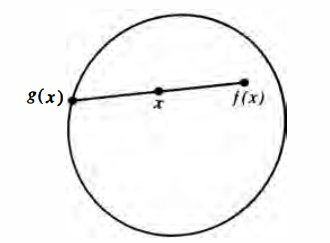
\includegraphics[width=0.6\textwidth]{Chapters/Brouwer Line.png}
    \end{center}

    If $x \in \partial B^n$, then $g(x) = x$. Thus, $g: B^n \to B^n$ is the identity on $\partial B^n$. If $g$ is smooth, then we get a contradiction to the above retraction theorem. Indeed, as $x$ is in the line segment between $f(x)$ and $g(x)$, we may write $g(x) - f(x)$ as $t(x - f(x))$ for some $t \geq 1$. Thus, $g(x) = tx + (1-t)f(x)$. If $t$ depends smoothly on $x$, then $g$ is smooth. By taking the dot porduct of both sides of this formula, and using the fact that $|g(x)| = 1$, we get that 
    \[t^2|x = f(x)|^2 + 2tf(x)[x-f(x)]+ |f(x)|^2 - 1 = 0\]
    This is a quadratic polynomial with a unique positive root. We can then use the quadratic formula to get an expression for $t$ in terms of smooth functions of $x$.
\end{proof}

\section{Transversality}

We know already that transversality is stable under perturbation for maps with compact domain. Using Sard's Theorem, we can prove a more general claim: any smooth $f: X \to Y$, regardless of behaviour with respect to $Z \subseteq Y$, can be deformed by some small amount to become transversal to $Z$. 

The key to this involves families of maps. Suppose $f_s: X \to Y$ is a family of smooth maps indexed by $s \in S$, and define $F: X \times S \to Y$ by $F(x,s) = f_s(x)$. 

\begin{theorem}[The Transversality Theorem]
    Suppose $F: X \times S \to Y$ is a smooth map of manifolds, where only $X$ has boundary, and let $Z$ be any boundaryless submanifold of $Y$. If both $F$ and $\partial F$ are transversal to $Z$, then for almost every $s \in S$, $f_s$ and $\partial f_s$ are transversal to $Z$.
\end{theorem}

\begin{proof}
    $W = F^{-1}(Z)$ is a submanifold of $X \times S$ with boundary $\partial W = W \cap \partial(X \times S)$. Let $\pi: X \times S \to S$ be projection to $S$. We claim that if $s \in S$ is a regular value of the restriction of $\pi$ to $W$, then $f_s \pitchfork Z$, and if $s$ is a regular value for the restriction of $\partial \pi$ to $\partial W$, then $\partial f_s \pitchfork Z$. By Sard's Theorem, almost all $s \in S$ are regular values of both maps, so the theorem follows. 
    
    We first show that $f_s \pitchfork Z$. Let $f_s(x) = z \in Z$. As $F(x,s) = z$ and $F \pitchfork Z$, we have that 
    \[dF_{(x,s)}T_{(x,s)}(X \times S) + T_z(Z) = T_Z(Y)\]
    so given $a \in T_z(Y)$, there is a $b \in T_{(x,s)}(X \times S)$ such that 
    \[dF_{(x,s)}(b) - a \in T_z(Z)\]
    We want to find a vector $v \in T_x(X)$ such that $df_s(v) - a \in T_z(Z)$. We know that 
    \[T_{(x,s)}(X \times S) = T_x(X) \times T_s(S)\]
    so $b = (w,e)$ for $w \in T_x(X), e \in T_s(S)$. If $e$ were 0 we'd be done, as the restriction of $F$ to $X \times \{s\}$ is $f_s$, so it follows that 
    \[dF_{(x,s)}(w,0) = df_s(w)\]
    So suppose that $e \neq 0$. We have that 
    \[d\pi_{(x,s)}: T_x(X) \times T_s(S) \to T_s(S)\]
    is projection to the second factor. $s$ is a regular value of $F$, so $d\pi_{(x,s)}$ maps $T_{(x,s)}(W)$ onto $T_s(S)$, there is a vector of the form $(u,e)$ in $T_{(x,s)}(W)$. But, $F: W \to Z$, so $dF_{(x,s)}(u,e) \in T_z(Z)$. Thus, taking $v = w - u$ gives us what we want, as 
    \[df_s(v) - a = dF_{(x,s)}[(w,e) - (u,e)] - a [dF_{(x,s)}(w,e) - a] - dF_s(u,e)\]
    with both of the latter vectors belonging to $T_z(Z)$. 

    A similar argument shows that $\partial f_s \pitchfork Z$ when $s$ is a regular value of $\partial \pi$. 
\end{proof}

This theorem easily shows that transversal maps are ``generic'' when $Y$ is a Euclidean space $\R^M$: If $f: X \to \R^M$ is smooth, let $S$ be an open ball of $\R^M$ and define $F: X \times S \to \R^M$ by $F_{(x,s)} = f(x) + s$. For $x \in X$, $F$ is a translation of $S$, clearly a submersion, so $F$ is a submersion of $X \times S$ and thus is transversal to any submanifold $Z$ of $\R^M$. By the Transversality Theorem, for almost all $s \in S$, $f_s(x) = f(x) + s$ is transversal to $Z$, so $f$ may be deformed into a transversal map simply by adding some small amount $s$. 

The proof for when $Y$ is a boundaryless manifold follows a similar nature. $Y$ lives in $\R^M$, and we showed how to vary a map $f: X \to Y$ through a family of maps carrying $X$ into $\R^M$. All that's left is to project these maps onto $Y$, obtaining suitable maps from $X$ into $Y$. Doing this requires us to know some some the geometry of $Y$ with respect to its environment. The compact case is clearest.

\begin{theorem}[$\varepsilon$-Neighbourhood Theorem]
    For a compact, boundaryless manifold $Y \subset \R^M$, and $\varepsilon > 0$, let $Y^\varepsilon$ be the set of points in $\R^M$ at most $\varepsilon$ away from $Y$. If $\varepsilon$ is small enough, each $w \in Y^\varepsilon$ has a unique closest point in $Y$, which we denote as $\pi(w)$. The map $\pi: Y^\varepsilon \to Y$ is a submersion. 

    If $Y$ is not compact, then there is still a submersion $\pi: Y^\varepsilon \to Y$ that is the identity on $Y$, but $\varepsilon$ is now a smooth positive function on $Y$, and
    \[Y^\varepsilon = \{w \in \R^M: |w - y|< \varepsilon(y) \text{ for some $y \in Y$}\}\]

    \begin{center}
        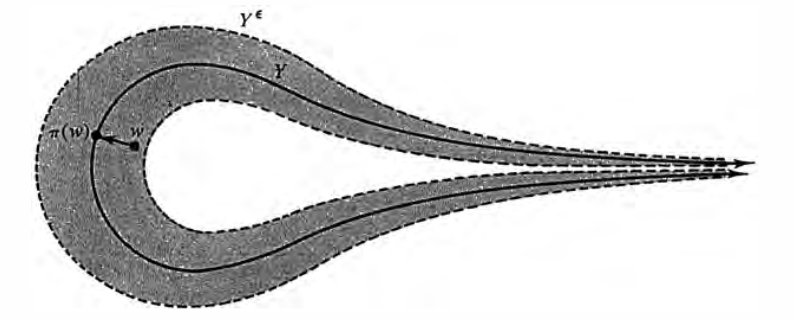
\includegraphics[width=0.7\textwidth]{Chapters/epsilon nbhd thm.png}
    \end{center}
\end{theorem}

We hold off on proving this for a moment to get some additional machinery. First a corollary:

\begin{corollary}
    Let $f: X \to Y$ be smooth, with $Y$ boundaryless. Then there is an open ball $S$ in some Euclidean space and a smooth map $F: X \times S \to Y$ such that $F(x,0) = f(x)$, and for any fixed $x \in X$, the map $s \mapsto F(x,s)$ is a submersion from $S$ into $Y$. In particular, $F,\partial F$ are submersions. 
\end{corollary}

\begin{proof}
    Let $S$ be the unit ball in $\R^M$ and define 
    \[F(x,s) = \pi[f(x) + \varepsilon(f(x))s]\]
    Since $\pi: Y^\varepsilon \to Y$ restricts to the identity on $Y$, $F(x,0) = f(x)$. For a fixed $x \in X$, we have that 
    \[s \mapsto f(x) + \varepsilon(f(x))s\]
    which is a submersion of $S$ into $Y$. As the composition of submersions is a submersion, $s \mapsto F(x,s)$ is a submersion. $F$ and $\partial F$ must be submersions, for they are even when restricted to $\{x\} \times S$, and one such submanifold passes through each point of $X \times S$, and each point of $(\partial X) \times S$. 
\end{proof}

The fact that transversality is generic follows directly. The form we need is as follows:

\begin{theorem}[Transversality Homotopy Theorem]
    For any smooth map $f: X \to Y$ and boundaryless submanifold $Z$ of the boundaryless manifold $Y$, there is a smooth map $g: X \to Y$ homotopic to $f$ such that $g \pitchfork Z$ and $\partial g \pitchfork Z$. 
\end{theorem}

\begin{proof}
    Take the family of mappings $F$ from the above corollary. The Transversality Theorem implies that $f_s \pitchfork Z$ and $\partial f_s \pitchfork Z$ for almost all $s \in S$. But, each $f_s$ is homotopic to $f$, with the homotopy given by $(x,t) \mapsto F(x,ts)$. 
\end{proof}

We will need another object as well, something similar to the tangent bundle. For each $y \in Y$, let $N_y(Y)$, called the \textbf{normal space of $Y$ at $y$}, be the orthogonal complement to $T_y(Y)$ in $\R^M$. Then the \textbf{normal bundle} $N(Y)$ is the set
\[\{(y,w) \in Y \times \R^M : v \in N_y(Y)\}\]
Notice that $N(Y)$ depends on the relationship between $Y$ and $\R^M$, unlike $T(Y)$. There is a projection map $\sigma: N(Y) \to Y$ defined by $\sigma(y,v) = y$. 

\begin{prop}
    If $Y \subset \R^M$, then $N(Y)$ is a manifold of dimension $M$ and the projection map $\sigma$ is a submersion
\end{prop}

\begin{proof}[Proof of the $\varepsilon$-Neighbourhood Theorem]
    Let $h: N(Y) \to \R^M$ be $h(y,v) = y + v$. $h$ is regular at all points of $Y \times \{0\}$ in $N(Y)$, for through $(y,0)$, there pass two natural complementary manifolds of $N(Y)$: $Y \times \{0\}$ and $\{y\} \times N_y(Y)$. The derivative of $h$ at $(y,0)$ maps $T_{(y,0)}(Y \times \{0\})$ onto $T_y(Y)$ and maps $T_{(y,0)}(\{y\} \times N_y(Y))$ onto $N_y(Y)$. Thus, it maps onto $T_y(Y) + N_y(Y) = \R^M$.

    As $h$ maps $Y \times \{0\}$ diffeomorphically onto $Y$ and is regular at each $(y,0)$, it maps a neighbourhood of $Y \times \{0\}$ diffeomorphically onto a neighbourhood of $Y$ in $\R^M$. Any neighbourhood of $Y$ contains some $Y^\varepsilon$, thus $h^{-1}: Y^\varepsilon \to N(Y)$, is defined, and $\pi = \sigma \circ h^{-1}: Y^\varepsilon \to Y$ is the desired submersion.
\end{proof}

A stronger version of the Transversality Homotopy Theorem is required. 

\begin{definition}
    A map $f: X \to Y$ is \textbf{transversal to $Z$ on a subset $C$ of $X$} if 
    \[df_xT_x(X) + T_{f(x)}(Z) = T_{f(x)}(Y)\]
    is satisfied for all $x \in C \cap f^{-1}(Z)$. 
\end{definition}

We need a lemma first:

\begin{lemma}
    If $U$ is an open neighbourhood of a closed set $C \subseteq X$, then there is a smooth function $\gamma: X \to [0,1]$ that is identically equal to tone outside $U$ but is zero on a neighbourhood of $C$. 
\end{lemma}

The proof is an application of partitions of unity.

\begin{theorem}[The Extension Theorem]
    Suppose that $Z$ is a closed submanifold of $Y$, both boundaryless, and $C \subseteq X$ is closed. Let $f: X \to Y$ be a smooth map with $f \pitchfork Z$ on $C$, and $\partial f \pitchfork Z$ on $C \cap \partial X$. Then there is a smooth map $g: X \to Y$ homotopic to $f$ such that $g \pitchfork Z$, and $\partial g \pitchfork Z$, and on a neighbourhood of $C$ we have that $g = f$. 
\end{theorem}

As the boundary of $X$ is closed in $X$, we also get a special case:

\begin{corollary}
    If for $f: X \to Y$, $\partial f: \partial X \to Y$ is transversal to $Z$, then there is a map $g: X \to Y$ homotopic to $f$ such that $\partial g = \partial f$ and $g \pitchfork Z$. 
\end{corollary}

In other words, if $h: \partial X \to X$ is transversal to $Z$ and extends to any map of $X \to Y$, then it extends to a map transversal to $Z$ on all of $X$. 

\section{Intersection Theory Mod 2}

We now apply the Transversality Lemma and other results from the previous section to develop an invariant for intersecting manifolds, which will give us some nice geometric complements. 

Two submanifolds $X,Z$ in $Y$ have \textbf{complementary dimension} if $\dim X + \dim Z = \dim Y$. If $X \pitchfork Z$, having complementary dimension makes $X \cap Z$ a zero-dimensional manifold (Note that we are now working without boundaries). If we further assume that $X,Z$ are closed, and that at least one of them is compact, say $X$, then $X \cap Z$ is a discrete set of points. For now, we could refer to the number of points in the intersection as the ``intersection number'' of $X,Z$, denoted $\#(X \cap Z)$. 

\begin{center}
    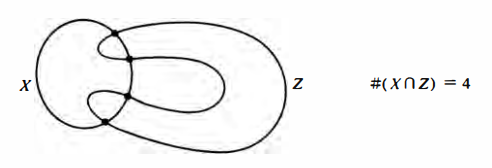
\includegraphics[width=0.4\textwidth]{Chapters/intersection number.png}
\end{center}

Can we generalize this to define intersection numbers for compact $X$ with an arbitary closed $Z$ of complementary dimension? Without transversality, the intersection could be some uncountable set of points, like a line. However, we can always deform $X$ slightly and make it transverse to $Z$. We could then define the intersection number as the that of the resulting two manifolds after this surgery. A problem seems to arise since there could be multiple intersection numbers, as shown here:
\begin{center}
    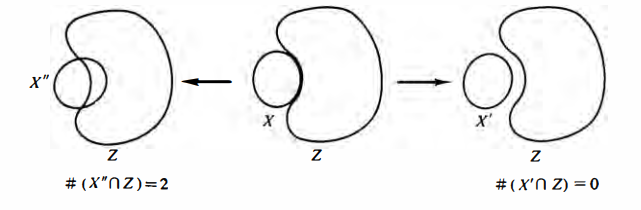
\includegraphics[width=0.5\textwidth]{Chapters/multiple intersection numbers.png}
\end{center}
However, we can still recover this, as these different intersection numbers will always agree \textit{mod 2}. Thus, we can define a mod 2 intersection number of $X$ and $Z$. 

Let's define the idea of deforming $X$ in a rigorous way. Let $X$ be an arbitary mainfold and consider the inclusion map $\iota: X \hookrightarrow Y$ as an embedding. We can deform $\iota$ by homotopy, and as embedding is stable, any homotopy of $\iota$ yields another embedding of $X$ into $Y$, producing an image manifold that is diffeomorphic to $X$. 

Suppose that $X$ is a compact manifold, not necessarily in $Y$, and let $f: X \to Y$ be smooth and transversal to some closed $Z$ in $Y$, where $\dim X + \dim Z = \dim Y$. Then $f^{-1}(Z)$ is a closed zero-dimensional submanifold of $X$, hence a finite set. We define the \textbf{mod 2 intersection number} of $f$ with $Z$, denoted $I_2(f,Z)$ as the number of points in $f^{-1}(Z)$, modulo 2. For any arbitary smooth map $g: X \to Y$, pick any map $f$ that is homotopic to $g$ and transversal to $Z$, and define $I_2(g,Z) = I_2(f,Z)$.

\begin{theorem}
    If $f_0,f_1: X \to Y$ are homotopic and transversal to $Z$, then their mod 2 intersection numbers are the same.
\end{theorem}

\begin{proof}
    Let $F: X \times I \to Y$ be a homotopy of $f_0,f_1$. By the Extension Theorem, we may assume that $F \pitchfork Z$. Since the boundary of $X \times I$ is equal to $X \times \{0\} \cup X \times \{1\}$, and $\partial F$ is $f_0$ on $X \times \{0\}$ and $f_1$ on $X \times \{1\}$, $\partial F \pitchfork Z$. Then $F^{-1}(Z)$ is a one-dimensional submanifold of $X \times I$ with boundary 
    \[\partial F^{-1}(Z) = F^{-1}(Z) \cap \partial (X \times I) = f_0^{-1}(Z) \times \{0\} \cup f_1^{-1}(Z) \times \{1\}\]
    From the classification of one-manifolds, this must have an even number of points. Thus, $\#f_0^{-1}(Z) = \#f_1{-1}(Z)$, mod 2.
\end{proof}

\begin{corollary}
    If $g_0,g_1: X \to Y$ are homotopic, then their mod 2 intersection numbers are equal.
\end{corollary}

We now return to the case that $X$ is compact in $Y$ and $Z$ is closed in $Y$ with complementary dimension. We define the mod 2 intersection number of $X$ with $Z$ as $I_2(X,Z) = I_2(\iota,Z)$, where $\iota$ is inclusion of $X$ into $Y$. When $X \pitchfork Z$, then $I_2(X,Z)$ is just $\#X \cap Z$ mod 2. If this value is not 0, then no matter how $X$ is deformed, we cannot pull it away from $Z$. As an example, on the torus $Y = S^1 \times S^1$, the complementary circles $S^1 \times \{1\}$ and $\{1\} \times S^1$ have non-zero mod 2 intersection numbers, and can never be pulled apart. 

What about when $\dim X$ is half that of $Y$? In this case, we can define the mod 2 \textbf{self-intersecting number} of $X$, $I_2(X,X)$. An example of this is the open M\"{o}bius band, which is just a strip where the ends have been half-twisted and taped together. If $X$ is just a line in the middle of the band, it has a mod 2 self-intersecting number of 1. Moreover, no matter how it is defromed, one can never pull it away from its original spot. 

If $X$ is the boundary of some manifold $W$ in $Y$, then $I_2(X,Z) = 0$, since if $Z \pitchfork X$, $Z$ must ``pass out'' of $W$ as often as it enters, hence the intersection number is even: 
\begin{center}
    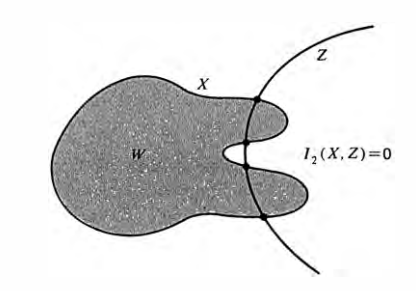
\includegraphics[width=0.5\textwidth]{Chapters/even intersection number.png}
\end{center}

\begin{theorem}[The Boundary Theorem]
    Suppose that $X$ is the boundary of some compact manifold $W$, and $g: X \to Y$ is smooth. If $g$ may be extended to all of $W$, then $I_2(g,Z) = 0$ for any closed submanifold of $Z$ in $Y$ of complementary dimensions. 
\end{theorem}

\begin{proof}
    Let $G: W \to Y$ extend $g$, with $\partial G = g$. From the Transversality Homotopy Theorem, we get a homotopic map $G: W \to Y$ with $F \pitchfork Z$ and $f = \partial F \pitchfork Z$. Then $f \sim g$, so $I_2(g,Z) = \#f^{-1}(Z) \mod 2$. But, $F^{-1}(Z)$ is a compact one-dimensional manifold with boundary, so $\#\partial F^{-1}(Z) = \# f^{-1}(Z)$ is even. 
\end{proof}

This gives us an good ``homotopy invariant'' on maps between manifolds of the same dimension:

\begin{theorem}
    If $f: X \to Y$ is smooth of a compact manifold $X$ into a connected manifold $Y$ with the same dimension as $X$, then $I_2(f,\{y\})$ is the same for all $y \in Y$.
\end{theorem}

\begin{proof}
    Let $y \in Y$. Then alter $f$ homotopically to make it transversal to $\{y\}$. By the Stack of Records Theorem, we have a neighbourhood $U$ of $y$ such that $f^{-1}(U)$ is a disjoint union $V_1 \cup \cdots \cup V_m$, where each $V_i$ is open in $X$ and mapped to $U$ diffeomorphically by $f$. We conclude that $I_2(f,\{z\}) = m$, mod 2, for all $z \in U$. Thus, the function defined on $Y$ that sends $y$ to $I_2(f,\{y\})$ must be locally constant. As $Y$ is connected, it must be constant globally. 
\end{proof}

This common value is called the \textbf{mod 2 degree of $f$}, denoted $\deg_2(f)$. Moreover, degree mod 2 is only defined when $Y$ is connected and $X$ is compact. 

Computing mod 2 degree of $f$ is actually really easy. Pick any regular value $y$ of $f$, and count its preimage points. $\deg_2(f) = \# f^{-1}(y)$ mod 2. Take for instance the map $z \to z^n$, which maps $S^1$ smoothly around itself $n$ times. It has mod 2 degree of 0 if $n$ is even, and 1 if $n$ is odd. mod 2 degree is an intersection number, so we get two theorems immediately:

\begin{theorem}
    Homotopic maps have the same mod 2 degree
\end{theorem}

\begin{theorem}
    If $X = \partial W$ and $f: X \to Y$ can be extended to all of $W$, then $\deg_2(f) = 0$.
\end{theorem}

We can apply this observation to investigate the zeroes of a function. Suppose that $p: \C \to \C$ is a smooth, complex function, and $W$ is a smooth compact region in the plane, which is a two-dimensional manifold with boundary. Does $p(z) = 0$ for some $z \in W$? 

Assume that $p$ has no zeroes on the boundary. Thus, the map $p/|p|: \partial W \to S^1$ is well-defined and smooth as a map of compact one-manifolds. If $p$ has no zeroes inside $W$, then we can define $p/|p|$ on all of $W$, and the last theorem then applies: 

\begin{prop}
    If the mod 2 degree of $p/|p|: \partial W \to S^1$ is non-zero, $p$ has a zero inside of $W$. 
\end{prop}

We can go even further and prove one half of the famous Fundamental Theorem of Algebra:

\begin{theorem}[Fundamental Theorem of Algebra: One Half]
    All complex polynomials of odd degree have a root
\end{theorem}

\begin{proof}
    Suppose that 
    \[p(z) = z^m + a_1z^{m-1} + \cdots a_m\]
    is a monic complex polynomial, and define a homotopy by 
    \begin{align*}
        p_t(z) & = tp(z) + (1-t)z^m \\
               & = z^m + t(a_1z^{m-1} + \cdots a_m)
    \end{align*}
    One can see that if $W$ is a closed ball of sufficiently large radiius, then none of the $p_t$ have zeroes on its boundary, as 
    \[\frac{p_t(z)}{z^m} = 1 + t\left(a_1 + \frac{1}{z} + \cdots + a_m \frac{1}{z^m}\right)\]
    and the term in the parenthesis goes to 0 as $z$ goes to infinity. Thus, the homotopy $p_t/|p_t|: \partial W \to S^1$ is defined for all of $t$, so we conclude that $\deg_2(p/|p|) = \deg_2(p_0/|p_0|)$. The polynomial $p_0$ is just $z^m$, so all points in $S^1$ have exactly $m$ preimage points on $W$'s boundary under $p_0/|p_0|$. Since we compute $\deg_2$ by computing preimages of regular values, $\deg_2(p_0/|p_0|) = m \mod{2}$. Then apply the proceeding proposition. 
\end{proof}

\section{The Borsuk-Ulam Theorem}

The following theorem is famous in topology:

\begin{theorem}[The Borsuk-Ulam Theorem]
    Let $f: S^k \to \R^{k+1}$ be smooth whose image does not contain the origin, and suppose that $f$ satisfies the symmetry condition that 
    \[f(-x) = -f(x) \quad \forall x \in S^k\]
    Then $W_2(f,0) = 1$, where $W_2(f,0)$ is the mod 2 winding number of $f$ around the origin. 
\end{theorem}

In natural language, this just means that any map that is symmetric about the origin must wind around it an odd number of times. 

\begin{proof}
    We proceed by induction on $k$. We leave the base case $k = 1$ as an exercise for the reader.

    Now, assume that the claim holds on $k - 1$, and let $f: S^k \to \R^{k+1}\setminus \{0\}$ be symmetric as described above. Embed $S^{k-1}$ into $S^k$ as the equator:
    \[(x_1,\ldots,x_k) \to (x_1,\ldots,x_k,0)\]
    
    Now denote the restriction of $f$ to the equator by $g$. Choose a suitable line $\ell$ such that, by Sard, we can pick a unit vector $\vec{a}$ that is regular for the maps
    \[\frac{g}{|g|}: S^{k-1} \to S^k, \quad \frac{f}{|f|}: S^k \to S^k\]
    By symmetry, $-\vec{a}$ is also regular for both maps. Comparing the dimensions, we see that the regularity of $g/|g|$ means that this function never hits $\vec{a}$ or $-\vec{a}$, and thus $g$ never intersects the line $\ell = \R \cdot \vec{a}$. Similarly, the regularity of $f/|f|$ means that $f \pitchfork \ell$. 

    Now, by definition, we have that 
    \[W_2(f,0) = \deg_2\left(\frac{f}{|f|}\right) = \#\left(\frac{f}{|f|}\right)^{-1}(a) \mod 2\]
    and due to symmetry, $f/|f|$ hits $\vec{a}$ just as often as $-\vec{a}$. Thus, 

    \[\#\left(\frac{f}{|f|}\right)^{-1}(a) = \frac{1}{2}\#f^{-1}(\ell)\]

    We compute this on the upper hemisphere. Let $f_+$ be the restriction to this hemisphere, $S_+^k$. By symmetry, plus the fact that the image of the equator under $f$ does not intersect $\ell$, we know that 
    \[\#f_+^{-1}(\ell) = \frac{a}{2}\#f^{-1}(\ell)\]
    We thus conclude taht $W_2(f,0) = \#f_+^{-1}(\ell) \mod 2$.

    The upper hemisphere is a manifold with boundary, and the boundary is $S^{k-1}$ where we can apply the induction hypothesis. Note that the dimensions don't match. To fix this, let $V$ be the orthogonal complement of $\ell$ and let $\pi: \R^{k+1} \to V$ be orthogonal projection. $g$ is symmetric and $\pi$ is linear, so $\pi \circ g: S^{k-1} \to V$ is symmetric; it is also never 0, since $g$ never intersects $\ell = \pi^{-1}(0)$. Identify $V$ with $\R^k$ and invoke induction hypothesis to get that $W_2(\pi \circ g, 0) = 1$. 

    Since $f_+ \pitchfork \ell$, 
    \[\pi \circ f_+: S_+^k \to V\]
    is transversal to $\{0\}$. Thus, we know that 
    \[W_2(\pi \circ g, 0) = \#(\pi \circ f_+)^{-1}(0)\]
    But,
    \[(\pi \circ f_+)^{-1}(0) = f_+^{-1}(\ell)\]
    so we have that 
    \[W_2(f,0) = \#f_+^{-1}(\ell) = W_2(\pi \circ g,0) = 1 \mod 2\]
    as required. 
\end{proof}

\begin{theorem}
    If $f: S^k \to \R^{k+1} \setminus \{0\}$ is symmetric about the orgin, then $f$ intersects every line through 0 at least once. 
\end{theorem}

\begin{proof}
    If $f$ never hits a line $\ell$, then use this $\ell$ in the above proof, whereby we obtain a contradiction that
    \[W_2(f,0) = \frac{1}{2}\#f^{-1}(\ell) = 0\]
\end{proof}

Borsuk-Ulam has many interesting consequences, which we describe below:

\begin{corollary}
    Any $k$ smooth functions $f_1,\ldots, f_k$ on $S^k$ that all satisfy the symmetry condition $f_i(-x) = -f_i(x)$ for all $i$, must possess a common zero.
\end{corollary}

\begin{proof}
    If not, we apply the above corollary to the map 
    \[f(x) = (f_1(x),\ldots,f_k(x),0)\]
    taking $\ell$ to be the $x_{k+1}$ axis. 
\end{proof}

\begin{theorem}
    For $k$ smooth functions $g_1,\ldots, g_k$ on $S^k$ there is a point $p \in S^k$ such that $g_i(p) = g_i(-p)$ for all $i$.
\end{theorem}

\begin{proof}
    Take $f_i(x) = g_i(x) - g_i(-x)$, then apply the above theorem. 
\end{proof}

A more physical formulation of this result is as follows: there must be two places on Earth that have the exact same weather and atmospheric pressure. 